\subsection{Bar charts}

\begin{frame}
\begin{center}
  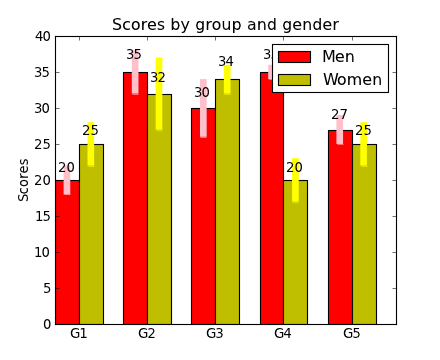
\includegraphics[scale=.5]{../figures/matplotlib/barchart_demo1.png}
\end{center}
\end{frame}

\begin{frame}[fragile]
\begin{block}{}
\begin{minted}{python}
N = 5
menMeans = (20, 35, 30, 35, 27)
menStd =   (2, 3, 4, 1, 2)

ind = np.arange(N)  # the x locations for the groups
width = 0.35       # the width of the bars

rects1 = bar(ind, menMeans, width,
         color='r',
         yerr=menStd,
         error_kw=dict(elinewidth=6, ecolor='pink'))
\end{minted}
\end{block}
\end{frame}

\begin{frame}[fragile]
\begin{block}{}
\begin{minted}{python}
womenMeans = (25, 32, 34, 20, 25)
womenStd =   (3, 5, 2, 3, 3)
rects2 = plt.bar(ind+width, womenMeans, width,
             color='y',
             yerr=womenStd,
             error_kw=dict(elinewidth=6, ecolor='yellow'))
\end{minted}
\end{block}
\end{frame}

\begin{frame}[fragile]
\begin{block}{}
\begin{minted}{python}
# add some
plt.ylabel('Scores')
plt.title('Scores by group and gender')
plt.xticks(ind+width, ('G1', 'G2', 'G3', 'G4', 'G5') )

plt.legend( (rects1[0], rects2[0]), ('Men', 'Women') )
\end{minted}
\end{block}
\end{frame}

\begin{frame}[fragile]
\begin{block}{}
\begin{minted}{python}
# add some
plt.ylabel('Scores')
plt.title('Scores by group and gender')
plt.xticks(ind+width, ('G1', 'G2', 'G3', 'G4', 'G5') )

plt.legend( (rects1[0], rects2[0]), ('Men', 'Women') )
\end{minted}
\end{block}
\end{frame}

\begin{frame}[fragile]
\begin{block}{}
\begin{minted}{python}
def autolabel(rects):
    # attach some text labels
    for rect in rects:
        height = rect.get_height()
        plt.text(rect.get_x()+rect.get_width()/2.,
                 1.05*height, '%d'%int(height),
                 ha='center', va='bottom')

autolabel(rects1)
autolabel(rects2)

plt.show()
\end{minted}
\end{block}
\end{frame}
